\documentclass[titlepage]{jsreport}

\usepackage[dvipdfmx]{graphicx}
\usepackage{listings}
\usepackage{url}

% ソースコードを挿入するための設定
\lstset{
 	language = Python,
     frame = tbrl
}

\title{卒業論文のタイトル}
\author{慶應義塾大学理工学部物理情報工学科\\
指導教員 渡辺宙志\\
学籍番号 61713173\\
内藤翔太}
\date{2020年MM月DD日}

\begin{document}

\maketitle

\tableofcontents

\chapter{はじめに} \label{chap:introduction}

「はじめに」もしくは「緒言」では、研究背景、目的、そして論文の構成を書く。

\section{研究の背景}

研究の背景は「なぜこの研究をしなければならないか」を、「大きい理由から小さい理由」へ書いていく。「大きい理由」は、「エネルギー問題」「安全」「便利」といった、「多くの人がほぼ納得するような理由」を挙げる。次に、その「大きな理由」を実現するために、これまでどのような試みがなされてきたかを説明する。これまでに読んだ論文のイントロダクションを参考に、必要な文献を引用しながら説得力のある文章を書くこと。

\section{研究の目的}

研究の背景を受けて、この研究分野は重要であるが、なんらかの不満点があることを述べる。その不満点は解決すべき問題であることを文献を引用しながら読者に納得させる。本研究の目的は、その不満点を解消することであることを述べ、その方法について簡単に述べる。

\section{本論文の構成}

論文の構成を説明する。まず本研究の目的を一行で書いてから、各章に何が書いてあるかを説明する。以下は例である。


本研究では、分野Aにおける手法Xの精度改善を行う。以下に本論文の構成を示す。第\ref{chap:introduction}章では、分野Aにおける手法の概観を紹介し、手法Xが広く用いられていることを示した。第\ref{chap:method}章では、本研究で用いる手法X、及びその改善手法であるX'について説明する。第\ref{chap:results}章では、本研究で提案した手法X'と、もととなった手法Xとの精度の比較を行う。第\ref{chap:summary}章では本研究で得られた知見を総括し、結論と今後の展望について述べる。




\chapter{手法} \label{chap:method}
\section{WCAポテンシャルの圧力}\label{method-sec:WCA-press}
\subsection{Weeks-Chandler-Andersen(WCA)ポテンシャル}\label{method-subsec:WCA}
分子動力学計算において頻繁に用いられるモデルの一つにLennard-Jones(以下LJ)ポテンシャルと呼ぶものが存在する。
このモデルにおいて、二つの原子間相互作用ポテンシャルエネルギーは

\large
\begin{equation}
\phi(r)=4{\varepsilon}\left(\left(\frac{\sigma}{r}\right)^{12}-\left(\frac{\sigma}{r}\right)^6\right)\label{eq:lj}
\end{equation}
\normalsize
と書ける\cite{WATANABE20191}。
ここで、rは原子間距離、${\sigma}$は原子直径の長さ、${\varepsilon}$はポテンシャルの深さを表す。

式(\ref{eq:lj})の一項目$4{\varepsilon}(\frac{\sigma}{r})^{12}$は原子間の斥力作用によるものであり、二項目$-4\varepsilon(\frac{\sigma}{r})^{6}$は原子間の引力作用によるものである。

このLJポテンシャルの斥力作用と引力作用が入れ替わる$r=2^{\frac{1}{6}}{\approx}1.12246$にカットオフ距離を設けたポテンシャルをWeeks-Chandler-Andersen(以下WCA)ポテンシャルと呼ぶ。
カットオフ距離とは、その距離内の原子間の相互作用のみを考慮するものであり、それ以上の距離での原子間の力を無視するもの\cite{WATANABE20191}である。
WCAポテンシャルにおけるポテンシャルエネルギーは、

\large
\begin{equation}
\phi(r) = \left\{ \begin{array}{ll}
    4{\varepsilon}\left(\left(\frac{\sigma}{r}\right)^{12}-\left(\frac{\sigma}{r}\right)^6\right) & (r\leq2^{\frac{1}{6}}) \\
    0 & (r>2^{\frac{1}{6}})\label{eq:wca}
\end{array} \right.
\end{equation}
\normalsize
と書くことが出来る\cite{doi:10.1063/1.2176675}。
したがって、WCAポテンシャルとは式(\ref{eq:wca})のように斥力作用と引力作用が入れ替わる$r=2^{\frac{1}{6}}$にカットオフ距離を設けることにより、二原子間の引力作用を無視し、斥力作用のみを考慮したポテンシャルである。

図{\ref{fig:dis-poen}にLJポテンシャルとWCAポテンシャルにおける原子間距離と原子間のポテンシャルエネルギーの関係を示す。
(図{\ref{fig:dis-poen}ではLJポテンシャルとWCAポテンシャルにおける原子間距離と原子間のポテンシャルエネルギーの違いを表すことだけを必要としたので、LJにカットオフ距離2.5を設けている)

\begin{figure}[htbp]
    \begin{center}
        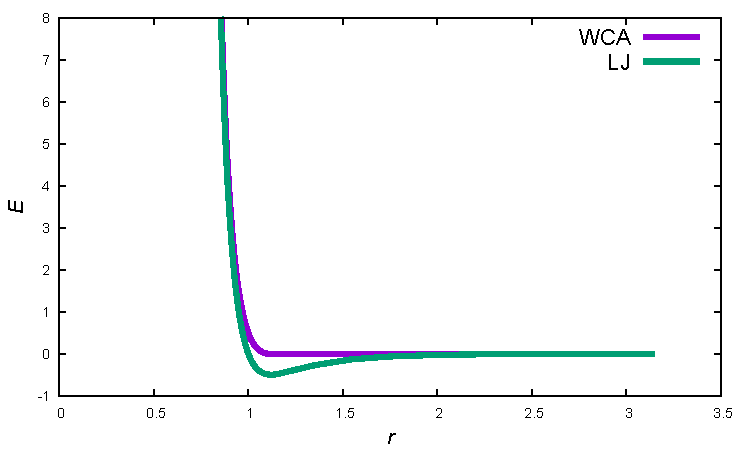
\includegraphics[width=13cm]{fig/dis-poen.pdf}
    \end{center}
    \caption{wcaとljの原子間距離-ポテンシャルエネルギーの関係}
    \label{fig:dis-poen}
\end{figure}


\subsection{WCAポテンシャルの相図}\label{method-subsec:WCA-phase}
相図とは、熱力学的な状態量と物質や系の関係を表したものであり、相図マッピングは、物理・成分科学の奥の分野で中心的な作業となっている\cite{phase-diagram}。
式(\ref{eq:wca})に示したWCAポテンシャルにおける相図を図\ref{fig:wca-phase-diagram}に示す。

\begin{figure}[htbp]
    \begin{center}
        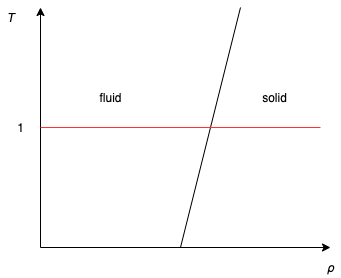
\includegraphics[width=9cm]{fig/wca-phase-diagram.png}
    \end{center}
    \caption{wcaの相図}
    \label{fig:wca-phase-diagram}
\end{figure}

\newpage
\subsection{WCAポテンシャルの圧力測定}\label{method-subsec:WCA-pressure}
式(\ref{eq:wca})に示したWCAポテンシャルにおける圧力の測定を分子動力学プログラムlammps\cite{lammps}によるシミュレーションを用いて行う。
尚、本研究では、式(\ref{eq:wca})の${\sigma}$(原子直径の長さ),${\varepsilon}$(ポテンシャルの深さ)を共に1とし、図\ref{fig:wca-phase-diagram}で示した赤線上の状態点について、研究を進めるものとする。(T=1.0)

本研究では、初期設定として1辺$L$の立方体の中に2048個の面心立方格子face-centered cubic(以下fcc)構造上に組んだ分子を仮定し、研究を進めるものとする。
以下に、初期状態の分子構造を示す。
*初期状態の分子構造をVMDで可視化し、挿入


この仮定から、用意されたWCAポテンシャルの数密度は、
\large
\begin{equation}
\rho = {\frac{2048}{L^3}}{\label{eq:density}}
\end{equation}
\normalsize
と求まる。

本研究では、数密度0.01〜15.0に0.01ずつ値をとり、lammpsにより圧力を測定した。
本研究では式(\ref{eq:density})にlammpsで指定した$L$を代入することにより数密度を決定するため、数密度を0にしてlammpsでシミュレーションを行うことが不可能であったため、数密度は0.01からとした。
ただし、数密度0では圧力が0であることは自明であるため、特に問題はないとする。
この初期条件のもと、温度制御を1.0とし、タイムステップ0.001で20000実行のシミュレーションを行った。
尚、全ての実験で温度制御ができていたことを前提とする。

WCAポテンシャルにおける圧力は、原子の1辺Lの立方体の壁への力と原子間の相互作用(斥力作用)による力に起因する。
この圧力は、ビリアル定理\cite{virial-therom}によって

\large
\begin{equation}
PV=NkT+{\frac{1}{3}}\langle\sum_{i=j}^N\vec{q_{ij}} \cdot \vec{r_{ij}}\rangle{\label{eq:Theoritical-pressure}}
\end{equation}
\normalsize
と書ける\cite{Theoritical-pressure}。
ここで、$P$は圧力、$V$は体積、$N$は原子数、$k$はボルツマン定数、$T$は温度、$\vec{q_{ij}}$は原子間距離、$\vec{r_{ij}}$は原子間に働く力である。

本研究では、lammpsによるシミュレーションで測定されたWCAポテンシャルの圧力の振る舞いを低密度(原子間の相互作用がない)、高密度、中密度において確認することを目的とする。

\section{WCAポテンシャルの状態方程式の推定}\label{method-sec:WCA-equation}
\subsection{ビリアル展開}\label{method-subsec:virial}
気体の振る舞いを表す有望な記述の一つにビリアル展開と呼ぶものが存在する。
これは、Heike Kamerlingh Onnesによって1901年に提唱されたもの\cite{virial-Heike}で、多くの研究で利用されている。
状態方程式のビリアル展開は、圧力を密度の冪級数を用いて表現するもので、

\large
\begin{equation}
P=b_1{\rho}+b_2{\rho}^2+b_3{\rho}^3+b_4{\rho}^4+\cdots \label{eq:virial}
\end{equation}

\normalsize
のように書くことが出来る。
式(\ref{eq:virial})の密度のn番目の累乗の係数を第nビリアル係数と呼ぶ\cite{virial-expansion}。
これらのビリアル係数は、増加する原子数で構成される集団群における原子の相互作用を表し、第2、第3、第4のビリアル係数は、2つ、3つ、4つ...の分子を含む衝突が気体中で重要になったときの理想的な振る舞いからの逸脱を表す。
圧力の効果は、分子間の距離を減少させることであるので、圧力が高くなるにつれて、考慮されなければならないビリアル項が増加する\cite{virial-Heike}。

\subsection{Benedict–Webb–Rubin(BWR)方程式}\label{method-subsec:BWR}
\ref{method-subsec:virial}のように、Heike Kamerlingh Onnesが提唱したビリアル展開は、圧力を密度の冪級数を用いて表現したものであるが、この式に経験則的に指数の項を付け加えたものをBenedict–Webb–Rubin(以下BWR)方程式と呼ぶ。
BWR方程式は、軽質炭化水素とその混合物の熱力学的特性を相関させ、予測するために1940年にBenedict Manson、Webb George B.、Rubin Louis C.によって提唱された\cite{BWR-equation:original}。
BWR方程式の原式は、圧力Pをモル密度dと絶対温度Tの関数として表現したもので、モル密度を$\rho$と表すことにすると、

\large
\begin{equation}
P=RT{\rho}+\left(B_0RT-A_0-{\frac{C_0}{T^2}}\right){\rho}^2+(bRT-a){\rho}^3+{\frac{c}{T^2}}(1+{\gamma}{\rho}^2)e^{-{\gamma}{\rho}^2}{\rho}^3+a{\alpha}{\rho}^6\label{eq:BWR}
\end{equation}
\normalsize
と書かれる。

BWR方程式は、気体の状態方程式を表すことに概ね成功していたが、厳密には純粋な物質や混合物の熱力学的性質を予測するのに十分とは言えなかった。
そこで、1973年には、Jacobsen Richard T.とStewart Richard B.によってBWR方程式の指数項をさらに増やした

\large
\begin{equation}
P=\sum_{n=1}^9a_n{\rho}^n+\exp(-{\gamma}{\rho}^2)\sum_{n=10}^{15}a_n{\rho}^{2n-17}\label{eq:mBWR}
\end{equation}
\normalsize
と書かれるmodified-Benedict–Webb–Rubin(以下mBWR)方程式が提唱\cite{m-BWR-equation}されたが、
依然として気体の状態方程式を完璧に再現することは出来なかった。
その後も、多くの研究者が気体の状態方程式の項を増やすことで、完璧な再現を試みた\cite{MCCARTY1974276}\cite{BWR-equation:13}\cite{BWR-equation:25}が、そのどれもが完璧な精度とは言えず、項の個数が増え続け、収集がつかなくなった。

\subsection{WCAポテンシャルの状態方程式の推定}\label{method-subsec:WCA-equation}
\ref{method-subsec:virial}、\ref{method-subsec:BWR}のように状態方程式を項を増やすことによって再現しようという試みは、項の個数が増え続け収集がつかなくなった。
また、BWR方程式の指数項は経験則的に付け加えたものであり、物理的意味もないことから項を増やし続け、状態方程式の再現をすることには意味がない。

そこで、本研究では、WCAポテンシャルにおける状態方程式をgnuplot\cite{gnuplot}のfittingにより表現することを目的とする。
gnuplotでのfittingは最小二乗法と呼ばれる方法で近似を行う。
以下最小二乗法の説明を入れる。

\section{Gaussian Process Regression(ガウス過程回帰)}\label{method-sec:Gauss}

ガウス過程回帰は、出力の不確実性も定量化できる確率的な補間予測を提供する\cite{machine-learning}ことができる。
ガウス過程回帰は、\cite{Gaussian-Processes-for-Machine-Learning}で開発された導出に従って、観測されたラベル$y$と予測されたラベル$y^*$の合同分布が

\large
\[
    \left[
        \begin{array}{l}
            y \\
            y^* 
        \end{array}
    \right]
    {\sim} N
    \left(0,
        \left[
            \begin{array}{cc}
                K(X,X) & K(X,X^*)\\    
                K(X,X^*) & K(X^*,X^*)
            \end{array}
        \right]
    \right)
\]
\normalsize

のようなガウスの事前分布に従う。


\section{引用の仕方}

原則として科学技術論文では、引用のない文章は「著者のオリジナル」であるとみなされる。LAMMPSなどのツールを使えばその関連論文を、手法の説明をするならその手法を提案した論文を引用しなければならない。

引用するのは、原則として書籍か査読論文とし、ウェブサイトの引用はさけること。特に何かの説明の参照先としてWikipediaやSlideShareなどを挙げないこと。機械学習の論文であればプレプリント(arXiv)を読むことも多いと思われるが、引用したくなるような論文はどこかのカンファレンスに採択されていることが多いので、そちらを引用すること。たとえ自分がWikipediaで知識を得たとしても、Wikipediaで引用されている文献にあたり、書籍なり論文なりを参考にすること。

参考文献は、原則としてBibTeXで管理すること。これにより、「本文で参照されていない文献を参考文献に入れてはならない」「本文で参照される順番に並べないとならない」などのルールが自動的に満たされる。

BibTeXでは、参考文献を「エントリ」と呼ばれる構造で管理する。エントリにはいくつか種別があるが、良く使うのは書籍(book)、論文(article)、プロシーディング(inproceedings)などであろう。例えば書籍は以下のようなエントリとする。

\begin{lstlisting}[language=TeX]
@book{okumura2020,
    author    = {奥村 晴彦 and 黒木 裕介},
    title     = {LaTeX2ε美文書作成入門},
    publisher = {技術評論社},
    year      = {2020}
}
\end{lstlisting}

これをTeXファイル中で以下のように引用する。

\begin{verbatim}
本論文の執筆にあたり、LaTeXの書き方については奥村・黒木の書籍を参考にした\cite{okumura2020}。
\end{verbatim}

これは以下のようにタイプセットされる。
\begin{quotation}
    本論文の執筆にあたり、LaTeXの書き方については奥村・黒木の書籍を参考にした\cite{okumura2020}。
\end{quotation}


GitHubのサイトなど、やむを得ずURLを引用する場合には、bibitemのmiscを使って以下のようにする。

\begin{lstlisting}[language=TeX]
@misc{github,
  howpublished = {\url{https://github.com/kaityo256/rbs}
},
\end{lstlisting}

例えば

\begin{verbatim}
この論文の参照実装はGitHubにて利用可能である\cite{github}。
\end{verbatim}
として引用すると、

\begin{quotation}
    この論文の参照実装はGitHubにて利用可能である\cite{github}。
\end{quotation}
となる。




\chapter{結果} \label{chap:results}

\section{WCAポテンシャルの圧力}\label{results-sec:WCA-press}
本研究では、lammpsによるシミュレーションで測定されたWCAポテンシャルの圧力の振る舞いを低密度(原子間の相互作用がない)、中密度、高密度において確認することを目的とする。

以下では、低密度(原子間の相互作用がない)状態、高密度状態、中密度状態において、具体的に見ていく。

\subsection{低密度(原子間の相互作用がない)状態のWCAポテンシャルの圧力}\label{results-sec:WCA-press-low-density}
本研究では、数密度0.01〜15.0に0.01ずつ値を取りlammpsによるシミュレーションで圧力を測定したが、カットオフ距離1.12246のWCAポテンシャルにおいて原子間の相互作用がない低密度(再隣接原子間距離$<$1.12246)状態では、
圧力は式(\ref{eq:Theoritical-pressure})の第一項のみを用いて、
\large
\begin{equation}
PV=NkT{\label{eq:ideal-gas}}
\end{equation}
\normalsize
と書けることが予測される。


式(\ref{eq:ideal-gas})より、
\large
\begin{eqnarray}
PV&=NkT\nonumber\\
{\Leftrightarrow}{\ }{\ }P&={\frac{N}{V}}kT\nonumber\\
{\Leftrightarrow}{\ }{\ }P&={\rho}kT\nonumber
\end{eqnarray}
\normalsize
と書け、本研究では、$k=1$、$T=1$として、lammpsのシミュレーションにより圧力測定を行ったので、

\large
\begin{equation}
P={\rho} \label{eq:ideal-value}
\end{equation}
\normalsize
と表されることを確認する。

式(\ref{eq:ideal-value})を「理論値」、本研究におけるlammpsのシミュレーションにより測定された圧力を「測定値」とし、その結果を図\ref{fig:lowden_compare:den-pre}に示す。

\begin{figure}[htbp]
    \begin{center}
        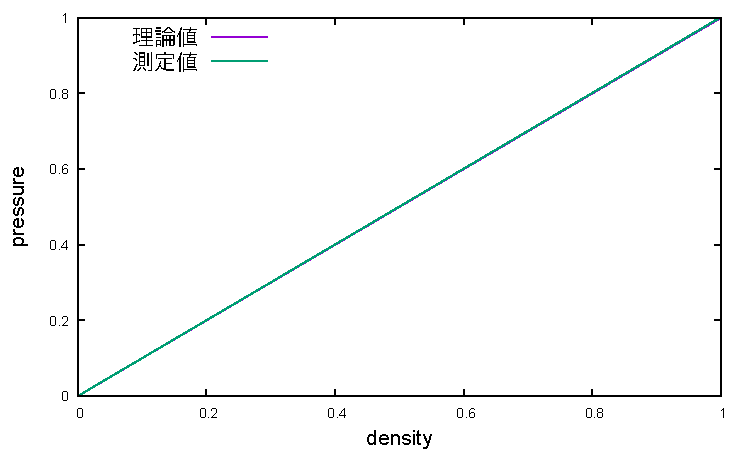
\includegraphics[width=14cm]{fig/lowden_compare:den-pre.pdf}
    \end{center}
    \caption{WCAポテンシャルの低密度における圧力の理論値と測定値の比較}
    \label{fig:lowden_compare:den-pre}
\end{figure}


図\ref{fig:lowden_compare:den-pre}から、原子間の相互作用がない低密度状態ではWCAポテンシャルの圧力は式(\ref{eq:ideal-gas})
と書けることがわかる。
これは、原子間の相互作用がない低密度状態では、原子が理想気体のように振る舞うことに依存する。

\subsection{高密度状態のWCAポテンシャルの圧力}\label{results-sec:WCA-press-high-density}
高密度状態では、圧力は式(\ref{eq:Theoritical-pressure})の第二項の影響を強く受ける。
高密度状態では、
密度が高くなればなるほど、式(\ref{eq:Theoritical-pressure})の第二項で考慮するものは、再隣接原子の寄与、第二隣接原子の寄与、第三隣接原子の寄与・・・と増えていく。

WCAポテンシャルにおいて原子間に働く力$\vec{r_{ij}}$の大きさは、
WCAポテンシャルのポテンシャルエネルギーが式(\ref{eq:wca})に従うことから、

\large
\begin{equation}
    | {\vec{r_{ij}}} |=\frac{d}{dr}\left(4\left(\left(\frac{1}{r}\right)^{12}-\left(\frac{1}{r}\right)^6\right)\right)=| 48r^{-13}-24r^{-7} |\label{eq:power}
\end{equation}
\normalsize
と書くことができるため、式(\ref{eq:Theoritical-pressure})の第二項の

\large
\begin{equation}
    \sum_{i=j}^N\vec{q_{ij}} \cdot \vec{r_{ij}} \label{eq:}
\end{equation}
\normalsize
は、距離に対して6乗で減衰することがわかる。

以上から、式(\ref{eq:Theoritical-pressure})の第二項への寄与はほとんどが再隣接原子であることから、本研究では、再隣接原子の寄与のみを考えるものとする。
第五隣接原子の寄与が生じる密度は、第五隣接原子間距離がWCAポテンシャルのカットオフ距離以下であればいいことから、
$\rho=14.697018915508458$と求まる。
これより高密度の状態では、次々に原子間の相互作用が働いていくが、この高密度状態でも圧力が式(\ref{eq:Theoritical-pressure})において
再隣接原子の寄与のみを考慮したもので十分に表されることを確認する。

式(\ref{eq:ideal-value})において再隣接原子の寄与のみを考慮したものを「理論値」、本研究におけるlammpsのシミュレーションにより測定された圧力を「測定値」とし、その結果を図\ref{fig:highden_compare:den-pre}に示す。

\begin{figure}[htbp]
    \begin{center}
        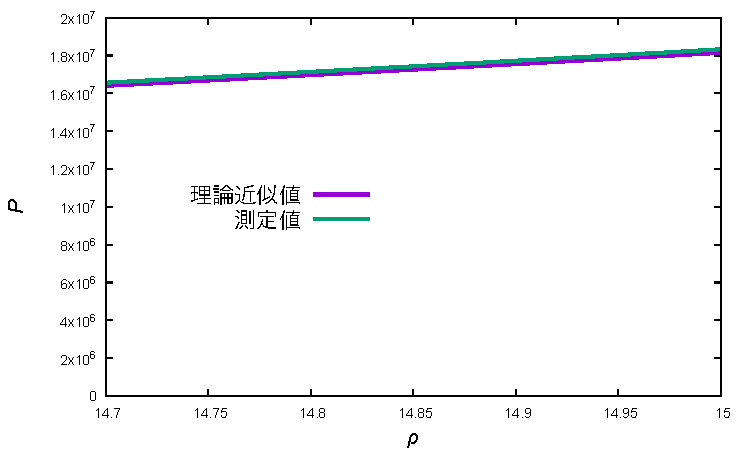
\includegraphics[width=14cm]{fig/highden_compare:den-pre.pdf}
    \end{center}
    \caption{WCAポテンシャルの高密度における圧力の理論値と測定値の比較}
    \label{fig:highden_compare:den-pre}
\end{figure}

図\ref{fig:highden_compare:den-pre}から、理論値と測定値のズレは1.2%以下であることがわかる。
このことから、第五隣接原子より離れた原子とも相互作用が働くほど高密度の状態でもWCAポテンシャルの圧力は式(\ref{eq:Theoritical-pressure})において
再隣接原子の寄与のみを考慮したもので十分に表されていることがわかる。

\subsection{中密度状態のWCAポテンシャルの圧力}\label{results-sec:WCA-press-middle-density}
中密度状態では、

以上を踏まえて、lammpsによるシミュレーションで測定されたWCAポテンシャルの圧力の振る舞いを確認できた。


\section{WCAポテンシャルの状態方程式}\label{results-sec:WCA-equation}
\ref{results-sec:WCA-press}節で見たように状態方程式を密度で展開する際、中密度すなわち、相転移近傍で困難を極める。
本研究では、WCAポテンシャルの状態方程式を機械学習を用いた関数近似を行うことにより表現することを目的とする。
まず、本研究で得られたlammpsのシミュレーションによる圧力の値を「測定値」、gnuplotを用いて5次式のfittingを行った関数を「5次式近似」とし、
\ref{fig:5den-pre}に示す。


\begin{figure}[htbp]
    \begin{center}
        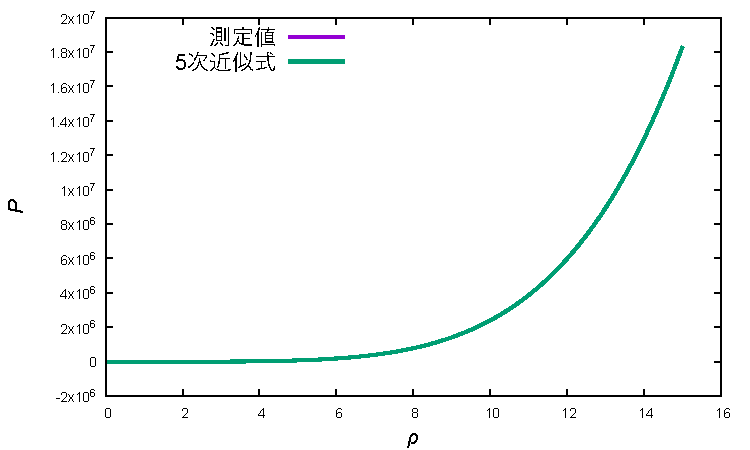
\includegraphics[width=14cm]{fig/5den-pre.pdf}
    \end{center}
    \caption{WCAポテンシャルの状態方程式の5次式近似}
    \label{fig:5den-pre}
\end{figure}



\section{ガウス過程回帰の精度}


\section{図の入れ方}

図は、数が多くなければとりえあずfigといったディレクトリにまとめて入れておくと良いだろう。数が増えてきて管理が難しくなったら節ごとにわけるなど工夫すること。画像ファイルは原則としてPDFにすること。例えば\verb|temperature.pdf|を入れたいなら、

\begin{lstlisting}[language=TeX]
    \begin{figure}[htbp]
        \begin{center}
            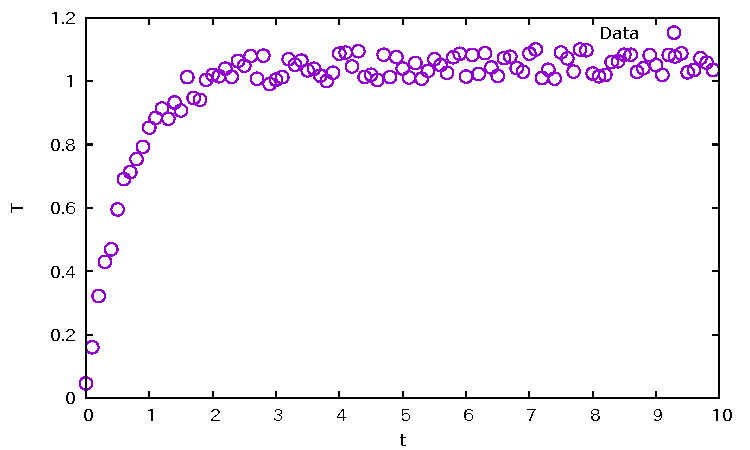
\includegraphics[width=10cm]{fig/temperature.pdf}
        \end{center}
        \caption{温度の時間発展。}
        \label{fig:temperature}
    \end{figure}
\end{lstlisting}

とすると、以下のような図が得られる。

\begin{figure}[htbp]
    \begin{center}
        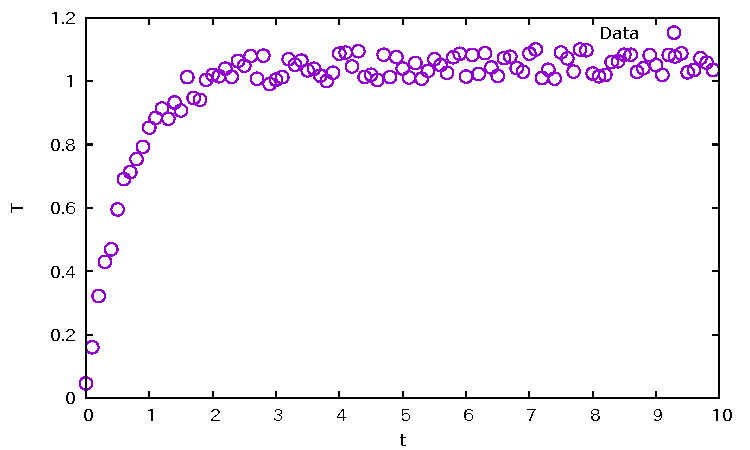
\includegraphics[width=10cm]{fig/temperature.pdf}
    \end{center}
    \caption{温度の時間発展。}
    \label{fig:temperature}
\end{figure}

この時、元データと、データからPDFを作るためのプロットファイルもしくはスクリプトファイルを一緒に入れておく。この時、画像ファイルとプロットファイルの名前を同じにしておくと良い。例えばgnuplotを使って\verb|temperature.pdf|という画像を作るなら、プロットファイルを\verb|temperature.plt|にしておく。すると、

\begin{lstlisting}[language=bash]
gnuplot temperature.plt
\end{lstlisting}

を実行することで\verb|temperature.pdf|ができるのでわかりやすい。

また、名前を揃えておくとmakefileとの相性が良くなる。例えば\verb|pressure.pdf|、\verb|temperature.pdf|、\verb|error.pdf|の三つのファイルが、同名のpltファイルから作成されるなら

\lstinputlisting[language=make]{fig/makefile}

といったmakefileを作っておけば、make一発で三つのファイルを作ることができるので便利だ。

もちろんPythonのMatplotlibを使っても良いが、いずれにせよ「データとスクリプトからコマンド一発で図のファイルが作成できる状況にしておく。

\chapter{考察および結論} \label{chap:summary}

考察は、「研究の背景」及び「目的」において提起した問題に正しく答えるようにする。得られた結果は満足すべきものだったか?不満があるならその理由はなにか?解決できそうなのか?また、「大きい理由」にも言及する。本研究によりどのような課題が見つかったかを書き、この分野における「研究の流れ」においてのような位置づけにあるかを説明した上で、今後、どのような発展の方向があるかについて書く。

\chapter*{謝辞}

まず、私を研究室に迎えれていただき、研究を進める上で、基礎的な部分から複雑な部分まで多くの指導をしていただいた渡辺宙志准教授には大変感謝しております。
研究部分のみならず、私たちの様子を常に気にかけ、研究設備や生活面でのサポートもしていただきましたこと心より御礼申し上げます。

また、同じ研究室に所属していた藤田くん、四辻くん、佐藤くんは、同じ部屋で研究を進め、分からない部分をお互いに共有しながら共に切磋琢磨できたと思います。
研究の合間に、昼ごはんを食べにいったり、他愛もない話をしたりと、息抜きをしながら研究を進めることが出来ましたこと、深く感謝致します。

最後に、研究のみならず、学生生活を様々な面でサポートしてくださった両親に深く感謝致します。


\appendix

\chapter{ソースコード}

\lstinputlisting[caption = 適当なPythonスクリプト, label = prog:sample]{src/sample.py}

\bibliographystyle{junsrt}
\bibliography{reference}

\end{document}